%!TeX root = ../SimplifyJapanese.tex
\begin{frame}[fragile]{Архитектура системы}%
  Система состоит из:
  \begin{enumerate}[1.]%
    \item Клиентского приложения. \\ 
      \notImportant{Написано на TypeScript + Lit, минималистичный дизайн с формой для ввода предложения на японском, ниже "--- вывод упрощённого варианта.}
    \item Сервера. \\ 
      \notImportant{Написан на Python + Falcon + MeCab, получает запрос с японским предложением, возвращает токены + упрощённый вариант.}
    \item Модели ИНС. \\
      \notImportant{Написана на Python + PyTorch + Spacy + HuggingFace, архитектура Transformer.}
  \end{enumerate}
\end{frame}


\begin{frame}[fragile]{Корпус SNOW}%
  Маруяма~Т. и Ямамото~К. вручную составили корпус из 85\,000 предложений с их упрощёнными вариантами.

  Словарь упрощённых предложений в корпусе составляет лишь 2\,000 слов.
  
  Корпус состоит из 2-х частей:
  \begin{enumerate}[1.]%
    \item SNOW 15: 50\,000 предложений (только обучение),
    \item SNOW 23: 35\,000 предложений (33\,000/1\,000/1\,000 "--- train/valid/test).
  \end{enumerate}
\end{frame}


\begin{frame}[fragile]{Пользовательское приложение}%
  Минималистичный дизайн: пользователь вводит предложение, нажимает Enter, снизу выводится его упрощённая версия.
  \begin{figure}[H]%
    \centering
    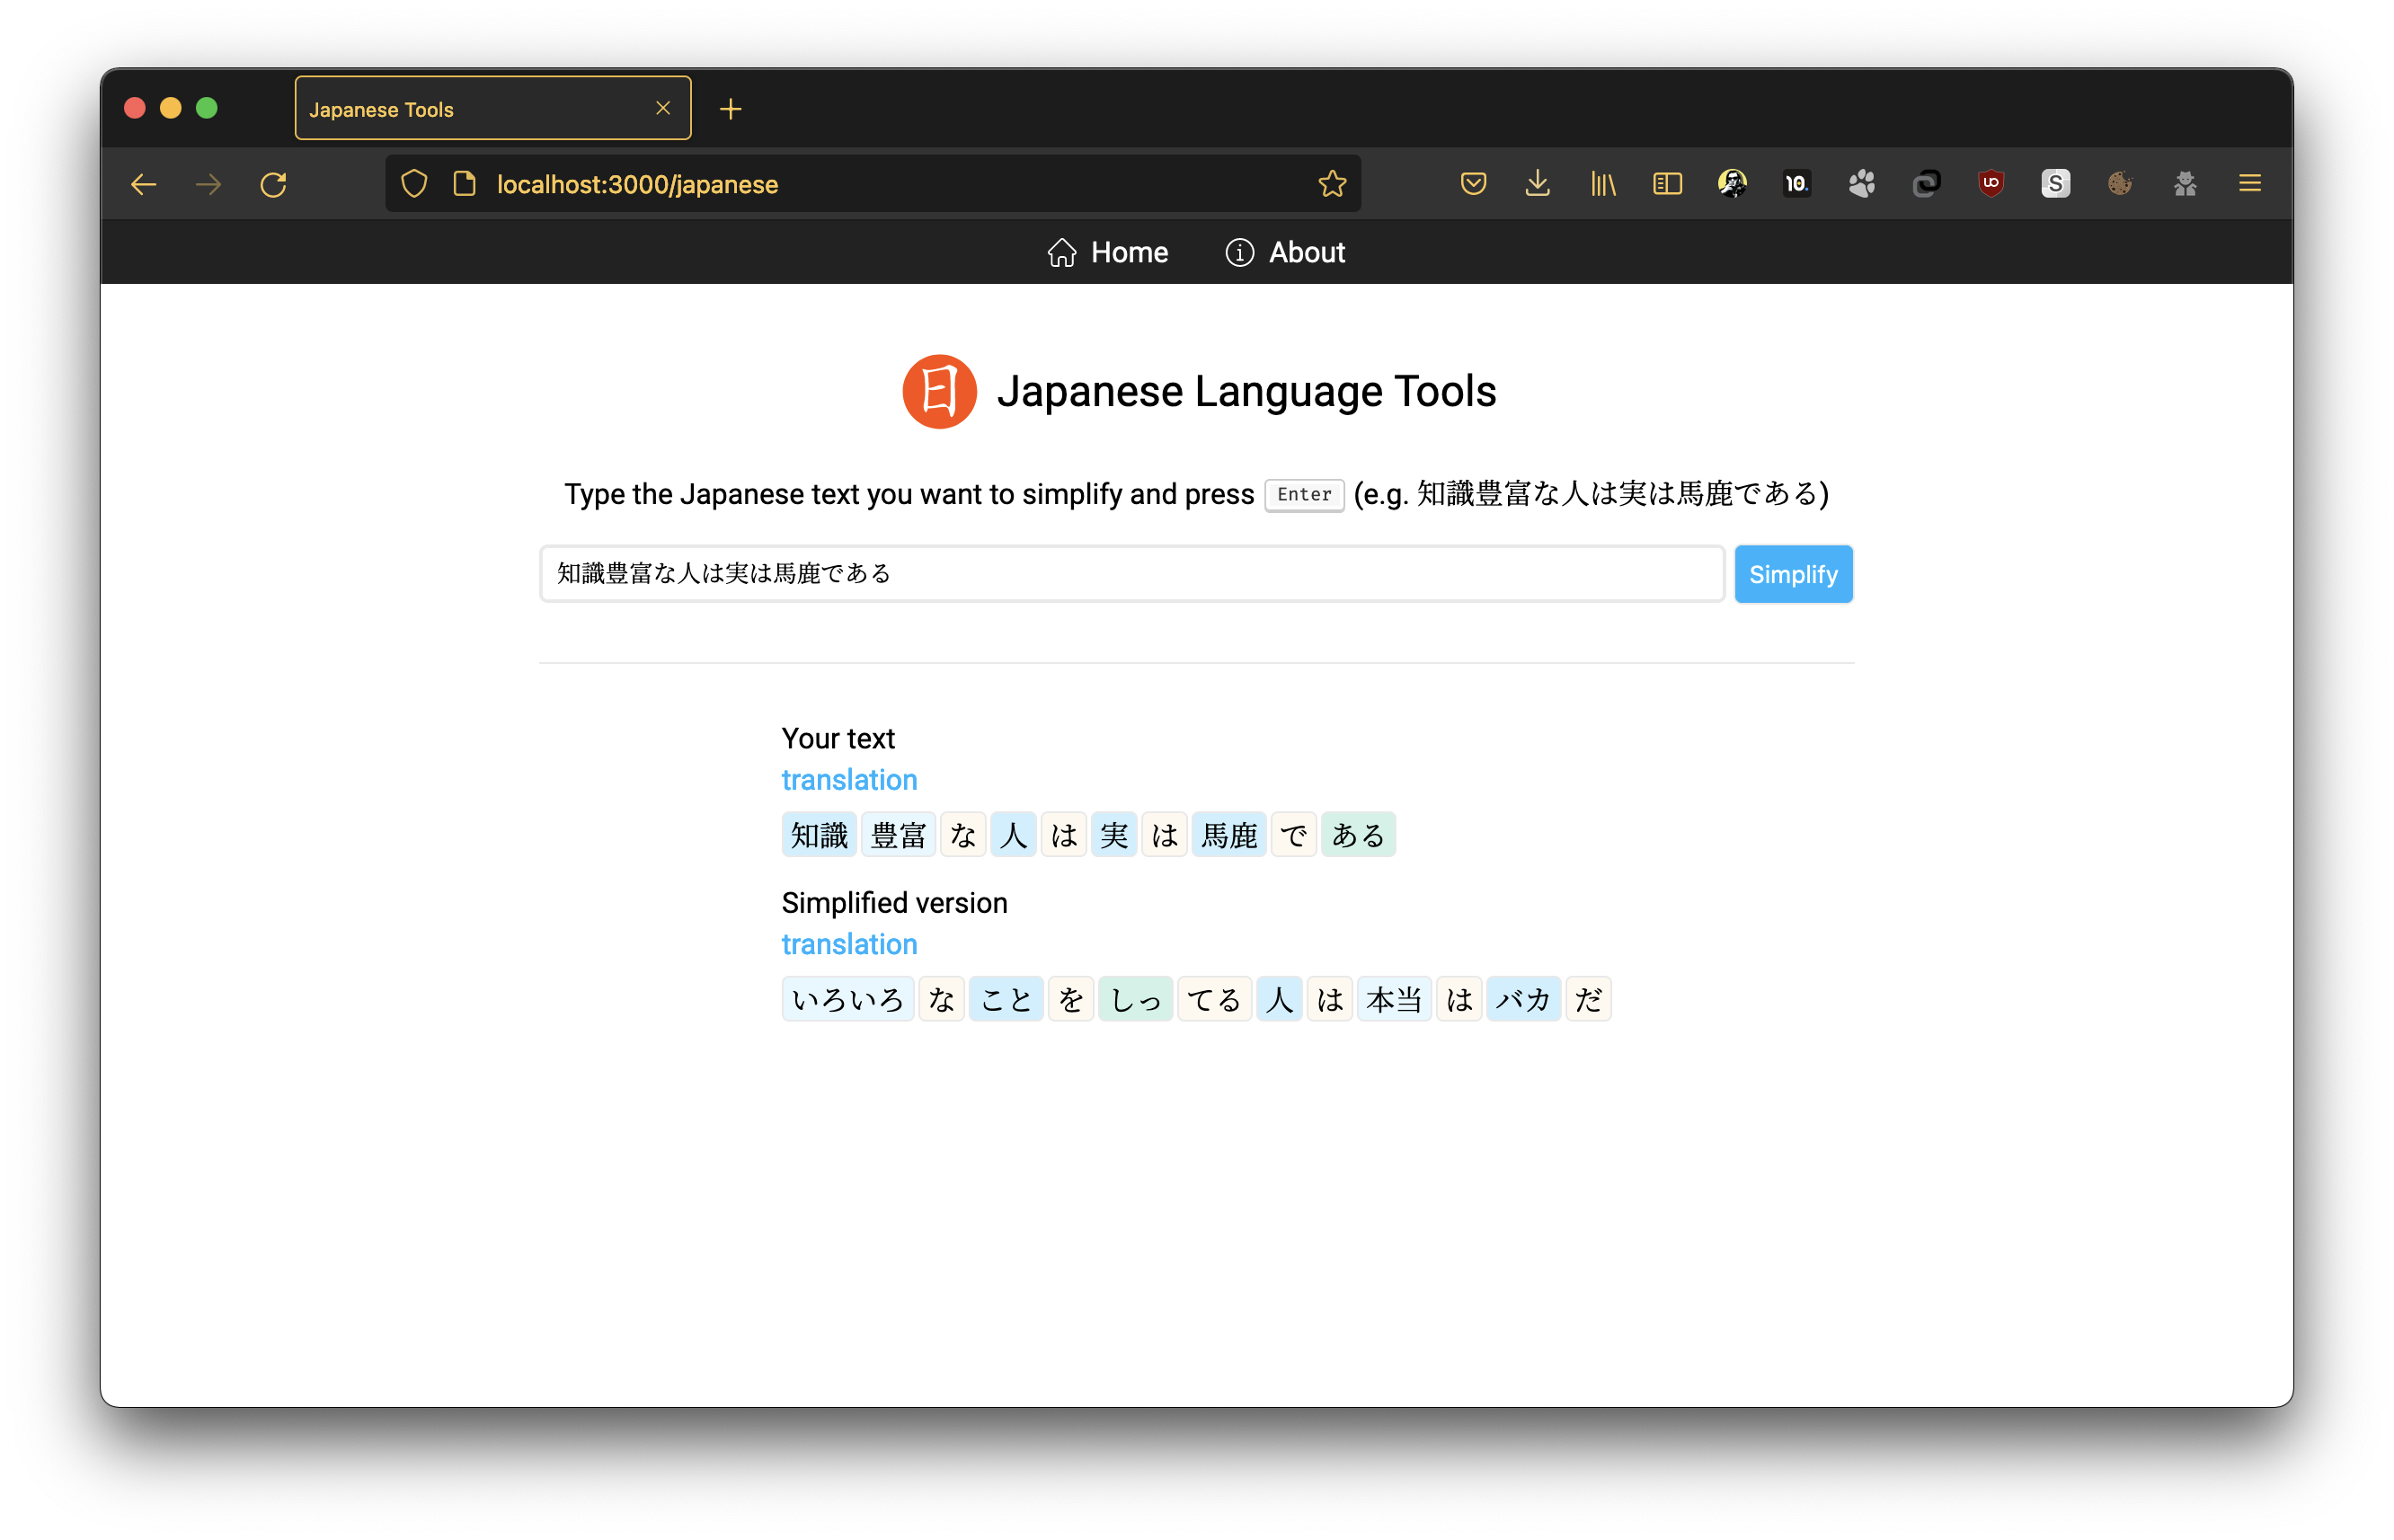
\includegraphics[width=0.6\textwidth]{app.png}
    \label{app-screen}
  \end{figure}
\end{frame}


\begin{frame}[fragile]{Проблемы реализованной системы}%
  Обученная модель обладает следующими недостатками:
  \begin{itemize}%
    \item плохо справляется с большими предложениями,
    \item имеет относительно небольшой «словарный запас».
  \end{itemize}

  Решение "--- предобучить \notImportant{(pretrain)} модель на неразмеченном корпусе и дообучить \notImportant{(fine-tune)} на корпусе SNOW:
  \begin{itemize}%
    \item Pretrained Transformer "--- предобучение всей модели,
    \item Pretrained Encoder "--- предобучение лишь encoder'а.
  \end{itemize}
\end{frame}
